%%%%%%%%%%%%%%%%%%%%%%%%%%%%%%%%%%%%%%%%%
% Beamer Presentation
% LaTeX Template
% Version 1.0 (10/11/12)
%
% This template has been downloaded from:
% http://www.LaTeXTemplates.com
%
% License:
% CC BY-NC-SA 3.0 (http://creativecommons.org/licenses/by-nc-sa/3.0/)
%
%%%%%%%%%%%%%%%%%%%%%%%%%%%%%%%%%%%%%%%%%

%----------------------------------------------------------------------------------------
% PACKAGES AND THEMES
%----------------------------------------------------------------------------------------

\documentclass[table, xcolor={dvipsnames}, 9pt]{beamer}
\usepackage{tikz}
\usetikzlibrary{positioning}
\mode<presentation> {

% The Beamer class comes with a number of default slide themes
% which change the colors and layouts of slides. Below this is a list
% of all the themes, uncomment each in turn to see what they look like.

%\usetheme{default}
%\usetheme{AnnArbor}
%\usetheme{Antibes}
%\usetheme{Bergen}
%\usetheme{Berkeley}
%\usetheme{Berlin}
%\usetheme{Boadilla}
%\usetheme{CambridgeUS}
%\usetheme{Copenhagen}
%\usetheme{Darmstadt}
%\usetheme{Dresden}
%\usetheme{Frankfurt}
%\usetheme{Goettingen}
%\usetheme{Hannover}
%\usetheme{Ilmenau}
%\usetheme{JuanLesPins}
%\usetheme{Luebeck}
% \usetheme{Madrid}
\usetheme{metropolis}
%\usetheme{Malmoe}
%\usetheme{Marburg}
%\usetheme{Montpellier}
%\usetheme{PaloAlto}
%\usetheme{Pittsburgh}
%\usetheme{Rochester}
%\usetheme{Singapore}
%\usetheme{Szeged}
%\usetheme{Warsaw}

% As well as themes, the Beamer class has a number of color themes
% for any slide theme. Uncomment each of these in turn to see how it
% changes the colors of your current slide theme.

%\usecolortheme{albatross}
%\usecolortheme{beaver}
%\usecolortheme{beetle}
%\usecolortheme{crane}
%\usecolortheme{dolphin}
%\usecolortheme{dove}
%\usecolortheme{fly}
%\usecolortheme{lily}
%\usecolortheme{orchid}
%\usecolortheme{rose}
%\usecolortheme{seagull}
%\usecolortheme{seahorse}
%\usecolortheme{whale}
%\usecolortheme{wolverine}

%\setbeamertemplate{footline} % To remove the footer line in all slides uncomment this line
%\setbeamertemplate{footline}[page number] % To replace the footer line in all slides with a simple slide count uncomment this line

%\setbeamertemplate{navigation symbols}{} % To remove the navigation symbols from the bottom of all slides uncomment this line
}

\usepackage{graphicx} % Allows including images
\usepackage{booktabs} % Allows the use of \toprule, \midrule and \bottomrule in tables
\usepackage{multirow}
\usepackage{natbib}
\usepackage[]{hyperref}
\usepackage{diagbox}
\usepackage{makecell}
\usepackage{subfig}
\usepackage{amsmath}
\usepackage{amsfonts,amsthm,amsmath,amssymb}    
\usepackage{bbm}
\usepackage{bm}
\usepackage{empheq}

\hypersetup{unicode=true,
            pdfusetitle,
            bookmarks=true,
            bookmarksnumbered=true,
            bookmarksopen=true,
            bookmarksopenlevel=2,
            breaklinks=false,
            pdfborder={0 0 1},
            backref=true,
            hypertexnames=false,
            pdfstartview={XYZ null null 1}}
\usepackage{xcolor}
\newcommand\myheading[1]{%
  \par\bigskip
  {\Large\bfseries#1}\par\smallskip}
\newcommand\given[1][]{\:#1\vert\:}
\theoremstyle{newstyle}
\newtheorem{thm}{Theorem}
\newtheorem{prop}[thm]{Proposition}
\newtheorem{lem}{Lemma}
\newtheorem{cor}{Corollary}
\newtheorem{defin}{Definition}
\newcommand*\diff{\mathop{}\!\mathrm{d}}
\newcommand*\Diff[1]{\mathop{}\!\mathrm{d^#1}}
\newcommand*{\QEDA}{\hfill\ensuremath{\blacksquare}}%
\newcommand*{\QEDB}{\hfill\ensuremath{\square}}%
\DeclareMathOperator{\E}{\mathrm{E}}
\DeclareMathOperator{\R}{\mathbb{R}}
\DeclareMathOperator{\Var}{\rm{Var}}
\DeclareMathOperator{\Cov}{\rm{Cov}}
\DeclareMathOperator{\e}{\rm{e}}
\DeclareMathOperator{\logit}{\rm{logit}}
\DeclareMathOperator{\indep}{{\perp\!\!\!\perp}}
%\DeclareMathOperator{\Pr}{\rm{Pr}}
\newenvironment{Column}[1][.5\linewidth]{\begin{column}{#1}}{\end{column}}
%----------------------------------------------------------------------------------------
% TITLE PAGE
%----------------------------------------------------------------------------------------

\title[]{Variance of the Difference-in-Means Estimator} % The short title appears at the bottom of every slide, the full title is only on the title page

\author{Thomas Leavitt} % Your name
\institute[] % Your institution as it will appear on the bottom of every slide, may be shorthand to save space
{
% Your institution for the title page
\medskip
\textit{} % Your email address
}
\date{\today} % Date, can be changed to a custom date

\begin{document}

\begin{frame}
\titlepage % Print the title page as the first slide
\end{frame}

%\begin{frame}
%\frametitle{Overview} % Table of contents slide, comment this block out to remove it
%\tableofcontents % Throughout your presentation, if you choose to use \section{} and \subsection{} commands, these will automatically be printed on this slide as an overview of your presentation
%\end{frame}

%------------------------------------------------------------------------
% PRESENTATION SLIDES
%------------------------------------------------------------------------
\section{Introduction}
\begin{frame}{Introduction}
\begin{itemize}
\item Our target is the ATE, which is equal to the expected value of the Difference-in-Means estimator \pause 
\item Variance tells us how far, on average, our estimator is from our target \pause 
\item We do not know the variance of the Difference-in-Means estimator \pause 
\item But we can conservatively estimate it \pause 
\item When combined with the finite population CLT, the conservative variance estimator facilitates tests of hypotheses about average causal effects
\end{itemize}
\end{frame}
%------------------------------------------------------------------------
\section{Variance of the Difference-in-Means Estimator}
\begin{frame}
\frametitle{Variance of Difference-in-Means estimator} 
\begin{itemize}
\item Consider again the ``village heads'' study from Gerber and Green (Chapter 2): \pause 
\item[]
\begin{center}
\begin{tabular}{l|rrr} \hline
& \multicolumn{3}{c}{Budget share (\%)} \\
Village &$y_{c}$& $y_{t}$& $\tau$  \\ \hline
1& 10 & 15  & 5  \\
2& 15 & 15  & 0   \\ 
3& 20 & 30  & 10   \\
4& 20 & 15  & -5   \\
5& 10 & 20  & 10   \\
6& 15 & 15  & 0   \\
7& 15 & 30  & 15   \\ \hline
Average & 15 & 20 & 5  \\ \hline
\end{tabular}
\end{center} \pause
\item[]
\item The target of interest is the \textit{average treatment effect}: \pause
\begin{align*}
\bar{\tau} & = \frac{1}{n}\sum \limits_{i = 1}^{n} \left(y_{ti} - y_{ci}\right) = \frac{1}{n}\sum \limits_{i = 1}^{n} \tau_i
\end{align*}
\end{itemize}
\end{frame}
%------------------------------------------------------------------------
\begin{frame}
\frametitle{Variance of Difference-in-Means estimator} 
\begin{itemize}
\item Yesterday we showed that the Difference-in-Means estimator for the ATE under complete random assignment is: \pause 
\item[]
\begin{figure}[H]
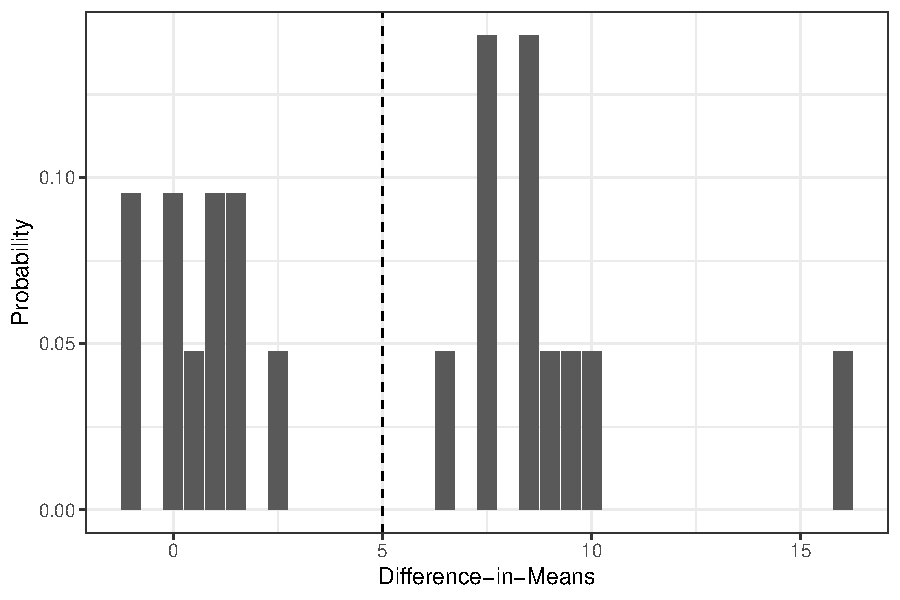
\includegraphics[width=0.9\linewidth]{cra_est_dist_plot.pdf}
\end{figure} \pause
\item What is the variance of this estimator? \pause 
\item Why do we care about variance of an estimator?
\end{itemize}
\end{frame}
%------------------------------------------------------------------------
\begin{frame}
\frametitle{Variance of Difference-in-Means estimator} 
\begin{itemize}
\item Intuitively, the variance of an estimator is the average squared distance of the estimator from its expected value: \pause 
\begin{itemize}
\item $\E\left[\left(t\left(\mathbf{Z}, \mathbf{Y}\right) - \E\left[t\left(\mathbf{Z}' \mathbf{Y}\right)\right]\right)^2\right]$ \pause 
\item Because the Difference-in-Means estimator is unbiased, i.e., $\E\left[t\left(\mathbf{Z}, \mathbf{Y}\right)\right] = \bar{\tau}$, we can write the estimator's variance as $\E\left[\left(t\left(\mathbf{Z}' \mathbf{Y}\right) - \bar{\tau}\right)^2\right]$
\end{itemize} \pause 
\item In the ``village heads'' example with 21 possible assignments under CRA, \pause 
\begin{align*}
\left(t\left(\mathbf{z}_1, \mathbf{y}_1\right) - \bar{\tau}\right)^2 \Pr\left(\mathbf{Z} = \mathbf{z}_1\right) + \ldots + \left(t\left(\mathbf{z}_{21}, \mathbf{y}_{21}\right) - \bar{\tau}\right)^2 \Pr\left(\mathbf{Z} = \mathbf{z}_{21}\right)
\end{align*} \pause 
\item The variance of the estimator in the ``village heads'' example under CRA is $\approx 21.19$
\end{itemize}
\end{frame}
%------------------------------------------------------------------------
\begin{frame}
\frametitle{Variance of Difference-in-Means estimator}
\begin{itemize}
\item Neyman (1923) derived an exact analytic expression for the variance of the Difference-in-Means estimator under CRA \pause 
\begin{equation}
\sigma^2_{\hat{\bar{\tau}}} = \frac{1}{n - 1}\left(\frac{n_1 \sigma^2_{y_c}}{n_0} + \frac{n_0 \sigma^2_{y_t}}{n_1} + 2\sigma_{y_c, y_t}\right),
\end{equation} \pause 
where $\sigma^2_{y_c}$ is the variance of control potential outcomes, \pause $\sigma^2_{y_t}$ is the variance of treated potential outcomes and \pause $\sigma_{y_c, y_t}$ is the covariance of control and treated potential outcomes \pause
\item In the ``village heads'' example, note that $n = 7$, $n_1 = 2$, $n_0 = 5$, $\sigma^2_{y_c} \approx 14.29$,  $\sigma^2_{y_t} \approx 42.86$, and $\sigma_{y_c, y_t} \approx 7.14$ \pause 
\item Hence, $\sigma^2_{\hat{\bar{\tau}}} \approx 21.19$
\end{itemize}
\end{frame}
%------------------------------------------------------------------------
\begin{frame}{Variance estimation} 
\begin{itemize}
\item In practice, we never actually know $\sigma^2_{y_c}$, $\sigma^2_{y_t}$ and $\sigma_{y_c, y_t}$ \pause 
\item We typically aim to estimate these unknown quantities from observed data \pause 
\item E.g., imagine we assign the $7$ villages to treatment and control and it just so happens that $\mathbf{z}' = (1, 0, 0, 0, 0, 0, 1)$ \pause
\item[]  
\item[]
\begin{center}
\begin{tabular}{lr|rrr} \hline
& & \multicolumn{3}{c}{Budget share (\%)} \\
Village & $z$ & $y_{c}$& $y_{t}$& $\tau$  \\ \hline
1& 1 & ?  & 15  & ?  \\
2& 0 & 15 & ?   & ?   \\ 
3& 0 & 20 & ?   & ?   \\
4& 0 & 20 & ?   & ?   \\
5& 0 & 10 & ?   & ?   \\
6& 0 & 15 & ?   & ?   \\
7& 1 & ?  & 30  & ?   \\ \hline
\end{tabular}
\end{center} \pause 
\item[]
\item We can unbiasedly and consistently estimate $\sigma^2_{y_c}$ and $\sigma^2_{y_t}$ from only partially observed potential outcomes \pause
\item However no such estimator exists for $\sigma_{y_c, y_t}$
\end{itemize}
\end{frame}
%------------------------------------------------------------------------
\section{Variance estimation}
\begin{frame}{Variance estimation} 
\begin{itemize}
\item Neyman (1923) proposed a conservative estimator: \pause 
\begin{itemize}
\item The maximum possible value of $2\sigma_{y_c, y_t}$ is $\sigma^2_{y_c} + \sigma^2_{y_t}$ \pause 
\item Substituting $\sigma^2_{y_c} + \sigma^2_{y_t}$ for $2\sigma_{y_c, y_t}$ and simple algebra yields \pause 
\begin{equation}
\frac{n}{n - 1}\left(\frac{\sigma^2_{y_c}}{n_0} + \frac{\sigma^2_{y_t}}{n_1}\right),
\end{equation} \pause 
\end{itemize}	
\item We can unbiasedly and consistently estimate this quantity via
\begin{equation}
\hat{\sigma}^2_{\hat{\bar{\tau}}} = \frac{n}{n - 1}\left(\frac{\hat{\sigma}^2_{y_c}}{n_0} + \frac{\hat{\sigma}^2_{y_t}}{n_1} \right),
\end{equation}
where \pause 
\begin{align*}
\hat{\sigma}^2_{y_c} & = \left(\frac{n - 1}{n\left(n_0 - 1\right)}\right)\sum \limits_{i: Z_i = 0}^n \left(y_{ci} - \hat{\mu}_{y_c}\right)^2 \\
\hat{\sigma}^2_{y_t} & = \left(\frac{n - 1}{n\left(n_1 - 1\right)}\right)\sum \limits_{i: Z_i = 1}^{n} \left(y_{ti} - \hat{\mu}_{y_t}\right)^2 \\ 
\hat{\mu}_{y_c} & = \left(\frac{1}{n_0}\right) \sum \limits_{i = 1}^n \left(1 - Z_i\right)y_{ci} \\ 
\hat{\mu}_{y_t} & = \left(\frac{1}{n_1}\right) Z_i y_{ti}
\end{align*}
\end{itemize}
\end{frame}
%------------------------------------------------------------------------
\begin{frame}{Variance estimation} 
\begin{itemize}
\item When potential outcomes are perfectly positively correlated, $\hat{\sigma}^2_{\hat{\bar{\tau}}}$ is unbiased and consistent; otherwise, positively biased (conservative) \pause 
\item[]
\item[]
\begin{figure}[H]
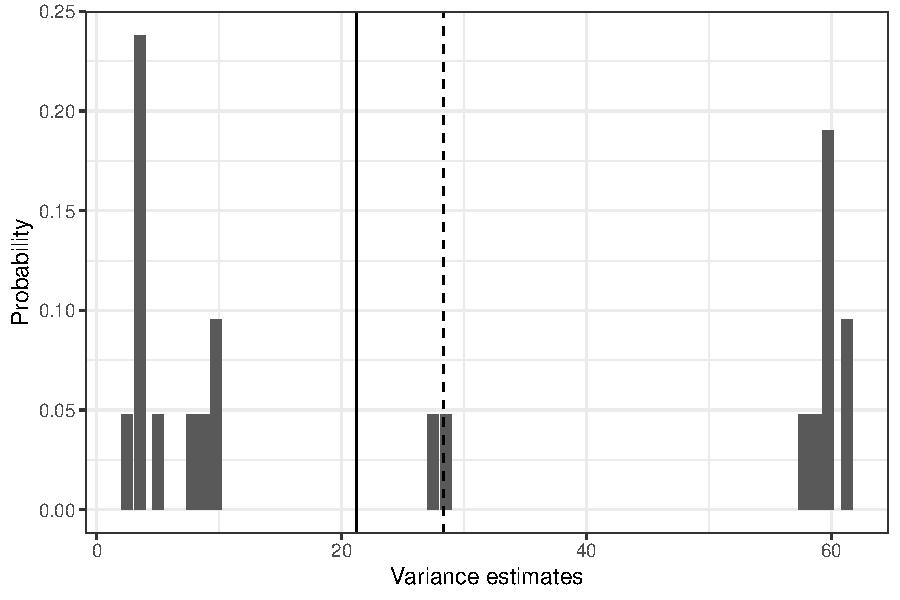
\includegraphics[width=0.8\linewidth]{cra_var_est_dist_plot.pdf}
\end{figure} \pause 
\item Solid line is true variance of Difference-in-Means estimator \pause 
\item Dashed line is expected value of conservative estimator of the Difference-in-Means estimator's variance
\end{itemize}
\end{frame}
%------------------------------------------------------------------------
\begin{frame}{Variance estimation}
\frametitle{}
\begin{itemize}
\item What happens as the experiment grows larger and larger? (See day 3 slides for notion of asymptotic growth) \pause 
\item[]
\item[]
\begin{figure}[H]
\includegraphics[width=\linewidth]{asymp_var_ests_plot.pdf}
\end{figure}
\end{itemize}
\end{frame}
%------------------------------------------------------------------------
\section{Hypothesis testing}
\begin{frame}{Hypothesis tests of the weak null}
\begin{itemize}
\item The finite population CLT tells us that 
\begin{align*}
\cfrac{\hat{\bar{\tau}} - \E\left[\hat{\bar{\tau}}\right]}{\sqrt{\sigma^2_{\hat{\bar{\tau}}}}} & \overset{d}{\to} \mathcal{N}\left(0, 1\right)
\end{align*} \pause 
\item Since the estimator is unbiased, a null hypothesis about $\E\left[\hat{\bar{\tau}}\right]$ is also a null hypothesis about $\bar{\tau}$ \pause 
\item We can plug in our conservative estimate $\hat{\sigma}^2_{\hat{\bar{\tau}}}$ for $\sigma^2_{\hat{\bar{\tau}}}$ \pause 
\item Calculate upper (u), lower (l) and two-sided (t) p-values as \pause 
\begin{align*}
p_u & =  1 - \Phi\left(\frac{\hat{\bar{\tau}} - \bar{\tau}_0}{\sqrt{\hat{\sigma}^2_{\hat{\bar{\tau}}}}}\right) \\
p_l & =  \Phi\left(\frac{\hat{\bar{\tau}} - \bar{\tau}_0}{\sqrt{\hat{\sigma}^2_{\hat{\bar{\tau}}}}}\right) \\
p_t & = 2\left(1 - \Phi\left(\frac{\left\lvert\hat{\bar{\tau}} - \bar{\tau}_0\right\rvert}{\sqrt{\hat{\sigma}^2_{\hat{\bar{\tau}}}}}\right)\right)
\end{align*}
\end{itemize}
\end{frame}
%------------------------------------------------------------------------
\begin{frame}{Hypothesis tests of the weak null}
\begin{itemize}
\item What do we make of the standard Normal approximation to $\cfrac{\hat{\bar{\tau}} - \E\left[\hat{\bar{\tau}}\right]}{\sqrt{\sigma^2_{\hat{\bar{\tau}}}}}$? \pause 
\item[]	
\item[]
\begin{figure}[H]
\includegraphics[width=\linewidth]{asym_stand_ests_plot.pdf}
\end{figure}
\end{itemize}
\end{frame}
%------------------------------------------------------------------------
\end{document}